\documentclass[border=3pt]{standalone}
% Preâmbulo compartilhado pelos diagramas TikZ da aula 11 (Localização por Grade e Monte Carlo)
\usepackage[T1]{fontenc}
\usepackage[utf8]{inputenc}
\usepackage{lmodern}
\usepackage{amsmath}
\usepackage{xcolor}
\usepackage{tikz}
\usetikzlibrary{arrows.meta,angles,quotes,decorations.pathmorphing,calc,
                positioning,shapes.geometric,shapes.misc,backgrounds,fit,
                math}

% Paleta (mesma dos SVGs originais)
\definecolor{dblue}{HTML}{2A5B8C}
\definecolor{dorange}{HTML}{B3541E}
\definecolor{dgreen}{HTML}{4A7C59}
\definecolor{dred}{HTML}{9C4B4B}
\definecolor{dcream}{HTML}{F4F1EA}
\definecolor{dshade}{HTML}{DDD7C9}

% Função gaussiana (não normalizada por padrão de escala visual)
\pgfmathdeclarefunction{gauss}{3}{%
  \pgfmathparse{1/(#3*sqrt(2*pi))*exp(-((#1-#2)^2)/(2*#3^2))}%
}

% Estilos comuns (prefixo d... para não colidir com chaves internas do pgf)
\tikzset{
  >={Stealth[length=2mm]},
  dguide/.style={gray!55, dashed, line width=0.4pt},
  daxis/.style={gray!60, line width=0.7pt, ->},
  dbody/.style={fill=black!3, draw=black!80, line width=1pt},
  dacc/.style={draw=dblue, line width=1pt},
  dlbl/.style={black!55, font=\small},
  dsub/.style={black!45, font=\footnotesize},
  dstate/.style={circle, draw=black!80, fill=dcream, line width=1pt,
                 minimum size=17mm, font=\large, inner sep=1pt},
  dobs/.style={circle, draw=black!80, fill=dshade, line width=1pt,
               minimum size=14mm, font=\large, inner sep=1pt},
  dbox/.style={rounded corners=2pt, draw=black!80, fill=dcream, line width=1pt,
               align=center, inner sep=6pt},
  dop/.style={circle, draw=black!80, fill=white, line width=1pt,
              minimum size=6mm, inner sep=0pt, font=\small},
  dtrans/.style={->, dblue, line width=1pt},
  dmeas/.style={->, dorange, line width=1pt},
  dcurve/.style={line width=1pt, dblue},
  dcurveb/.style={line width=1.4pt, dorange},
}

\begin{document}
\hyphenpenalty=10000 \exhyphenpenalty=10000 \tolerance=9999 \emergencystretch=3em
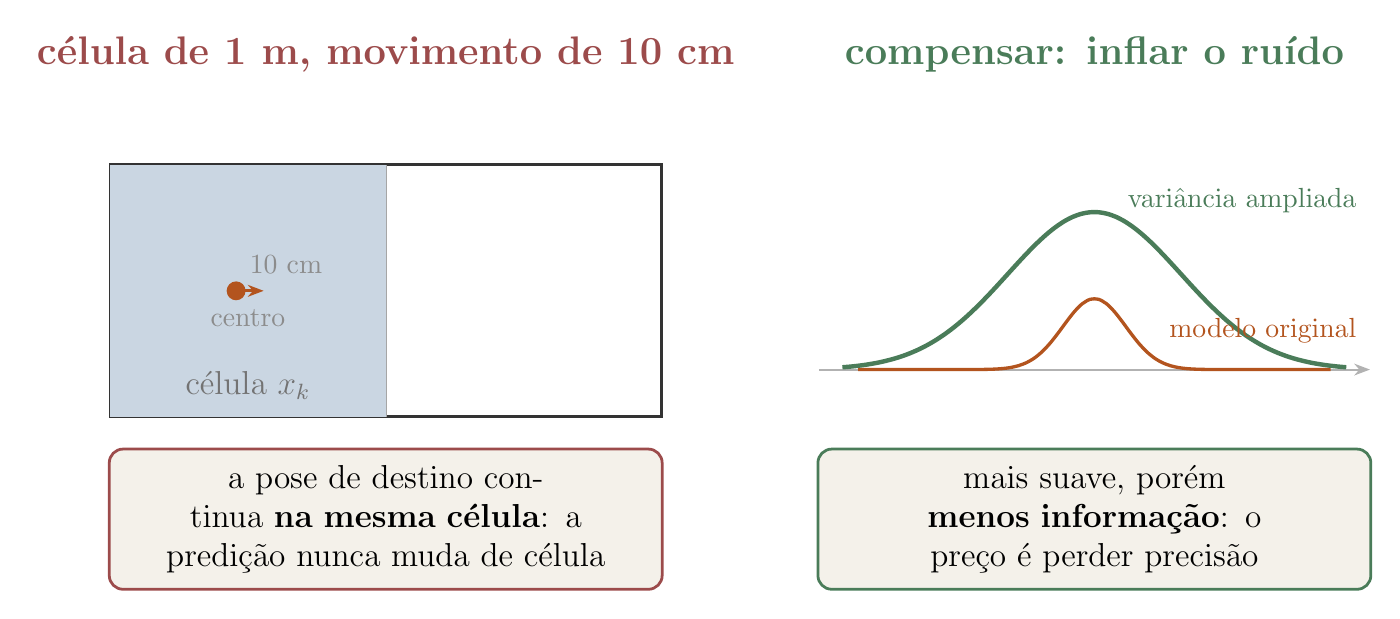
\begin{tikzpicture}[x=1cm,y=1cm]
  % painel A: problema
  \node[font=\Large\bfseries, dred] at (3.5,5.0) {célula de 1 m, movimento de 10 cm};
  \draw[dbody, fill=white, line width=1pt] (0,0.4) rectangle (7,3.6);
  \draw[black!35, line width=0.6pt] (3.5,0.4) -- (3.5,3.6);
  \fill[dblue!25] (0,0.4) rectangle (3.5,3.6);
  \fill[dorange] (1.6,2.0) circle (0.12); \node[dsub, font=\normalsize] at (1.75,1.65) {centro};
  \draw[dorange, ->, line width=1.2pt] (1.6,2.0) -- (1.95,2.0);
  \node[dsub, font=\normalsize, anchor=south west] at (1.65,2.1) {10 cm};
  \node[dlbl, font=\large] at (1.75,0.8) {célula $x_k$};
  \node[dbox, rounded corners=5pt, draw=dred, text width=6.6cm, font=\large] at (3.5,-0.9) {a pose de destino continua \textbf{na mesma célula}: a predição nunca muda de célula};
  % painel B: solução
  \begin{scope}[shift={(9,0)}]
    \node[font=\Large\bfseries, dgreen] at (3.5,5.0) {compensar: inflar o ruído};
    \draw[daxis] (0,1.0) -- (7,1.0);
    \draw[dorange, line width=1.2pt, domain=0.5:6.5, samples=60, smooth] plot (\x, {1.0+0.9*exp(-((\x-3.5)^2)/(2*0.4^2))});
    \draw[dgreen, line width=1.6pt, domain=0.3:6.7, samples=60, smooth] plot (\x, {1.0+2.0*exp(-((\x-3.5)^2)/(2*1.1^2))});
    \node[dorange, font=\normalsize, anchor=east] at (6.95,1.5) {modelo original};
    \node[dgreen, font=\normalsize, anchor=east] at (6.95,3.15) {variância ampliada};
    \node[dbox, rounded corners=5pt, draw=dgreen, text width=6.6cm, font=\large] at (3.5,-0.9) {mais suave, porém \textbf{menos informação}: o preço é perder precisão};
  \end{scope}
\end{tikzpicture}
\end{document}
